\newpage
\song{Hlavně že jsme na vzduchu (Z. SVěrák, J. Uhlíř)}
\begin{multicols}{2}

\ve
\ch{C}Když radosti není dosti,\\
\ch{F}raduju se z maličkostí.\\
\ch{C}Představím si \ch{Ami}třeba kdyby\\
\ch{G}lidi žili jako ryby.\\
To je \ch{C}dobře náho\ch{Emi}dou,\\
že ne\ch{C}{ž}ijem pod vo\ch{C}dou.\\
Na vzdu\ch{Emi}chu, na vzdu\ch{F}chu,\\
můžem \ch{G}zpívat ejchu\ch{C}chu.\\
\ch{G}Zpíva\ch{C}ti si pod vo\ch{Emi}dou,\\
nejde \ch{F}ani náho\ch{C}dou.\\
Z hlubi\ch{Emi}ny, z hlubi\ch{F}ny,\\
vyšly \ch{G}by jen bubli\ch{C}ny.\\

\vfill\columnbreak\vspace*{\fill}

\ve{}
To je dobře náhodou,\\
že nežijem pod vodou.\\
Na vzduchu, na vzduchu,\\
můžem zpívat ejchuchu.\\
Zpívati si pod vodou,\\
nejde ani náhodou.\\
Z hlubiny, z hlubiny,\\
vyšly by jen bubliny.\\
Jen si představ milá babi,\\
že jsme dejme tomu krabi.\\
Nebyla bys mou babičkou,\\
byla bys mořskou krabičkou.\\

\cho{}
Buďme rádi Bohouši,\\
že žijeme na souši.\\
Na zemi, na zemi,\\
ušmudlané sazemi.\\
Vžij se rybě do kůže,\\
třeba ti to pomůže.\\
I když jsi na suchu,\\
hlavně že jsi na vzduchu!\\

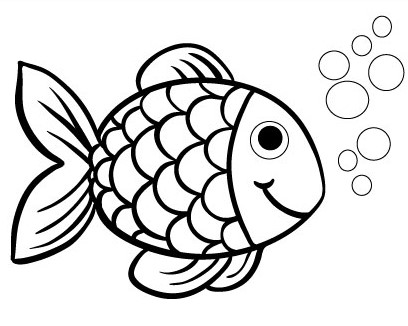
\includegraphics[width = \columnwidth]{images/hlavne_ze_sme_na_vzduchu.jpg}

\end{multicols}
\esong
